%!TEX root = mainfile.tex
\subsection{Tracking the circles}
\begin{figure}
\centering
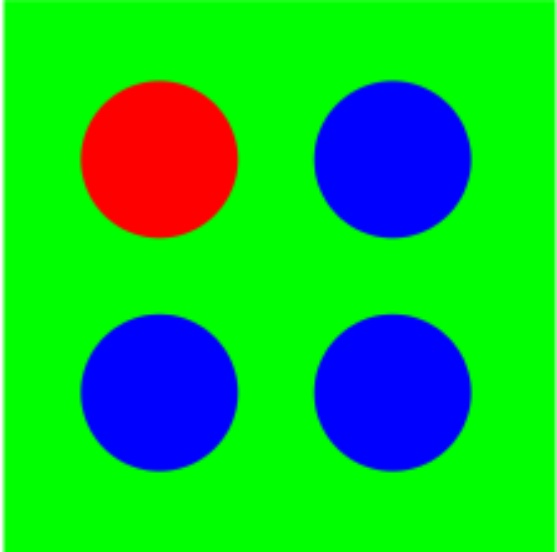
\includegraphics[width=0.3\textwidth]{circle_image_8}
\caption{The circle marker used for tracking}
\label{fig:original_circle_marker}
\end{figure}

In order to track the circles it is necessary to find them first.
A flowchart over the preparation and circle identification process can be seen in Figure~\vref{fig:circles_flowchart},
while examples during processing can be seen in Figure~\vref{fig:circle_process_examples}.
In order to find the circles the image is first converted to a grayscale image.
Next, it is put through the OpenCV function \verb|adaptiveThreshold| in order to get a binary image.
By using \verb|adaptiveThreshold| it is the difference between the pixels in a neighborhood that leeds to the thresholding,
rather than having to use color segmentation.
It is not clear if this method is actually faster than channel-based thresholding.
But it works.

%!TEX root = mainfile.tex
\begin{figure}
\centering
\begin{tikzpicture}[node distance=2cm,scale=0.6, every node/.style={transform shape}]
    \node (start) [startstop] {Start};
    \node (imgin) [io, below of=start] {Image in};
    \node (prepimg) [process, below of=imgin] {Grayscale, adaptive threshold, open, threshold, find contours};
    \node (contproc) [process, below of=prepimg] {Get new contour};
    \node (decarea) [decision, below of=contproc, yshift=-1.6cm] {Is area of contour > 1000?};
    \node (areaproc) [process, below of=decarea, yshift=-1.6cm] {Store contour};
    \node (decmore) [decision, below of=areaproc, yshift=-1.5cm] {More contours?};
    \node (sort) [process, right of=imgin, xshift=8cm] {Sort contours based on area-perimeter ratio};
    \node (takefour) [process, below of=sort] {Take four best circles based on ratio};
    \node (takered) [process, below of=takefour] {Take most red element as red circle};
    \node (takeopposite) [process, below of=takered, yshift=-.25cm] {Take contour with biggest center-to-center distance to red circle as opposite of red};
    \node (takeothers) [process, below of=takeopposite, yshift=-.25cm] {Take other two, assign based on algorithm};
    \node (calc) [process, below of=takeothers] {Calculate center point};
    \node (stop) [startstop, below of=calc] {Stop};
    \draw [arrow] (start) -- (imgin);
    \draw [arrow] (imgin) -- (prepimg);
    \draw [arrow] (prepimg) -- (contproc);
    \draw [arrow] (contproc) -- (decarea);
    \draw [arrow] (decarea) -| node[anchor=north east] {No} ([xshift=0.50cm]contproc.south east) |- (contproc);
    \draw [arrow] (decarea) -- node[anchor=east] {Yes} (areaproc);
    \draw [arrow] (areaproc) -- (decmore);
    \draw [arrow] (decmore) -| node[anchor=north west] {Yes} ([xshift=-0.50cm]contproc.south west) |- (contproc);
    \draw [arrow] (decmore) -| node[anchor=north east] {No} ([xshift=1.5cm]contproc.south east) |- (sort);
    \draw [arrow] (sort) -- (takefour);
    \draw [arrow] (takefour) -- (takered);
    \draw [arrow] (takered) -- (takeopposite);
    \draw [arrow] (takeopposite) -- (takeothers);
    \draw [arrow] (takeothers) -- (calc);
    \draw [arrow] (calc) -- (stop);
\end{tikzpicture}
\caption{Loading of image and detection and identification of circles.}
\label{fig:circles_flowchart}
\end{figure}


\begin{figure}[ht]
\centering
\begin{subfigure}[b]{0.3\linewidth}
\centering
    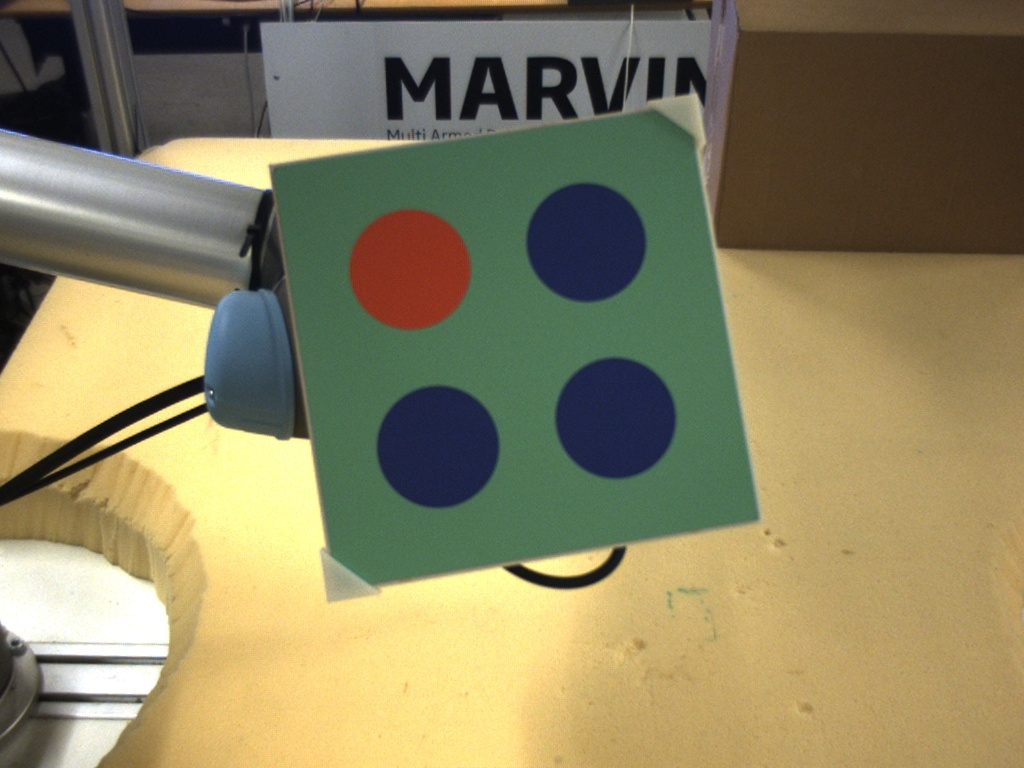
\includegraphics[width=0.8\textwidth]{circle_image_1}
    \caption{Original image}
\label{fig:circle_process_examples_1}
\end{subfigure}
\begin{subfigure}[b]{0.3\linewidth}
\centering
    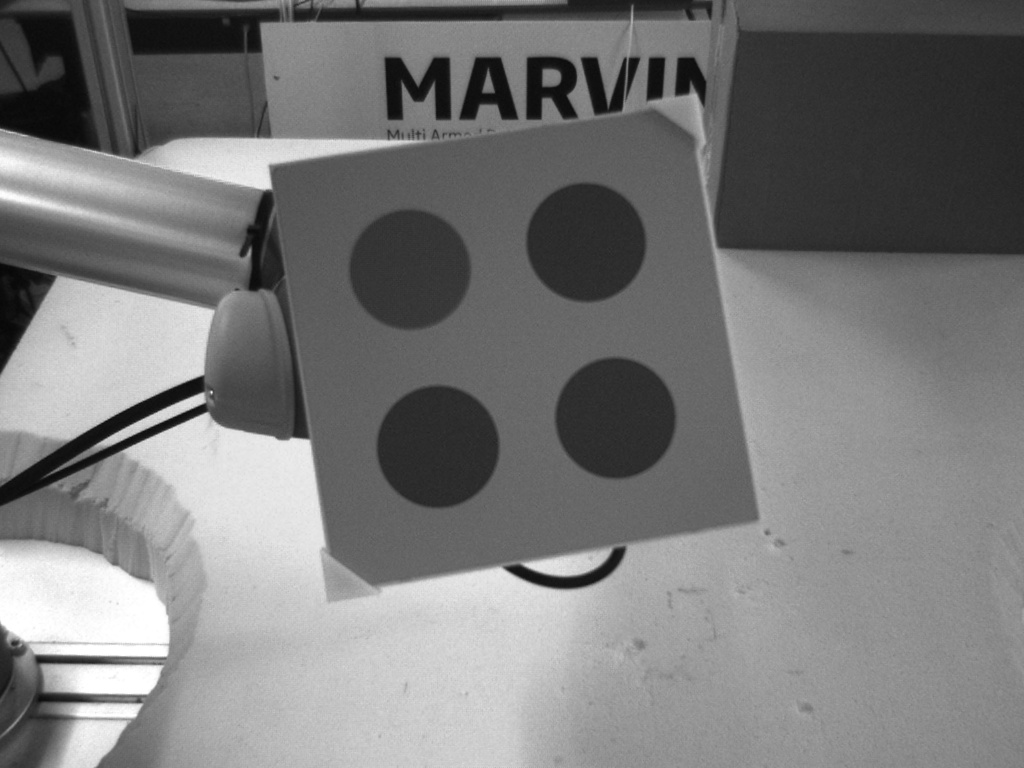
\includegraphics[width=0.8\textwidth]{circle_image_2}
    \caption{Grayscaled image}
\label{fig:circle_process_examples_2}
\end{subfigure}
\begin{subfigure}[b]{0.3\linewidth}
\centering
    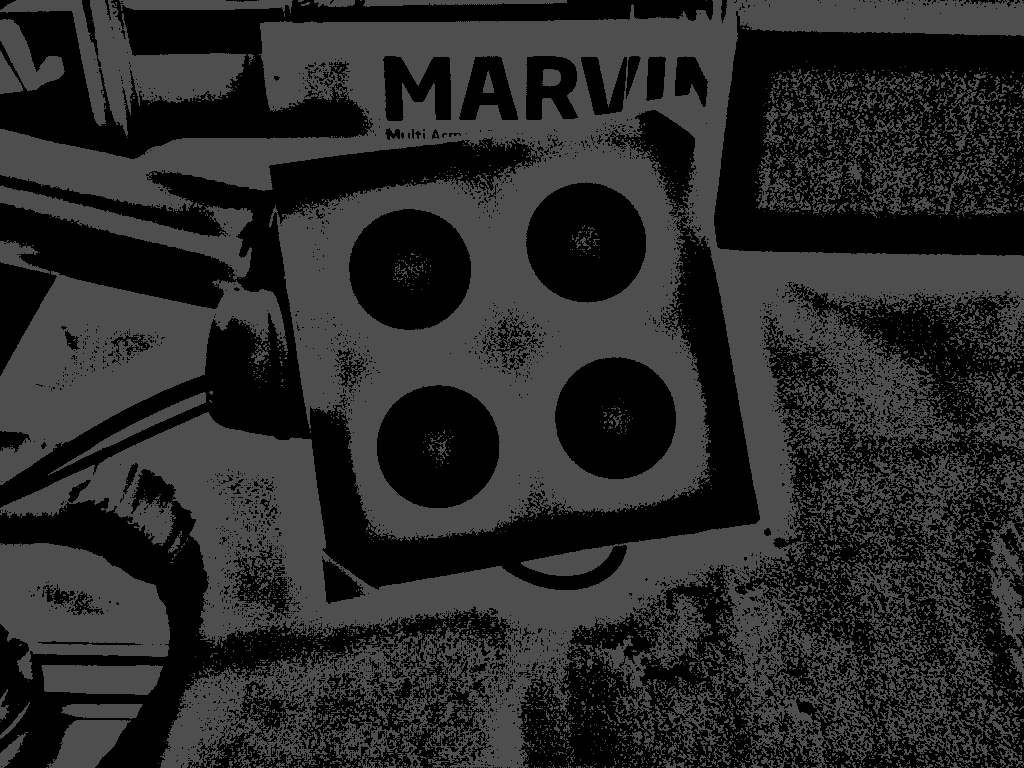
\includegraphics[width=0.8\textwidth]{circle_image_3}
    \caption{Adaptive threshold}
\label{fig:circle_process_examples_3}
\end{subfigure}\\
\begin{subfigure}[b]{0.3\linewidth}
\centering
    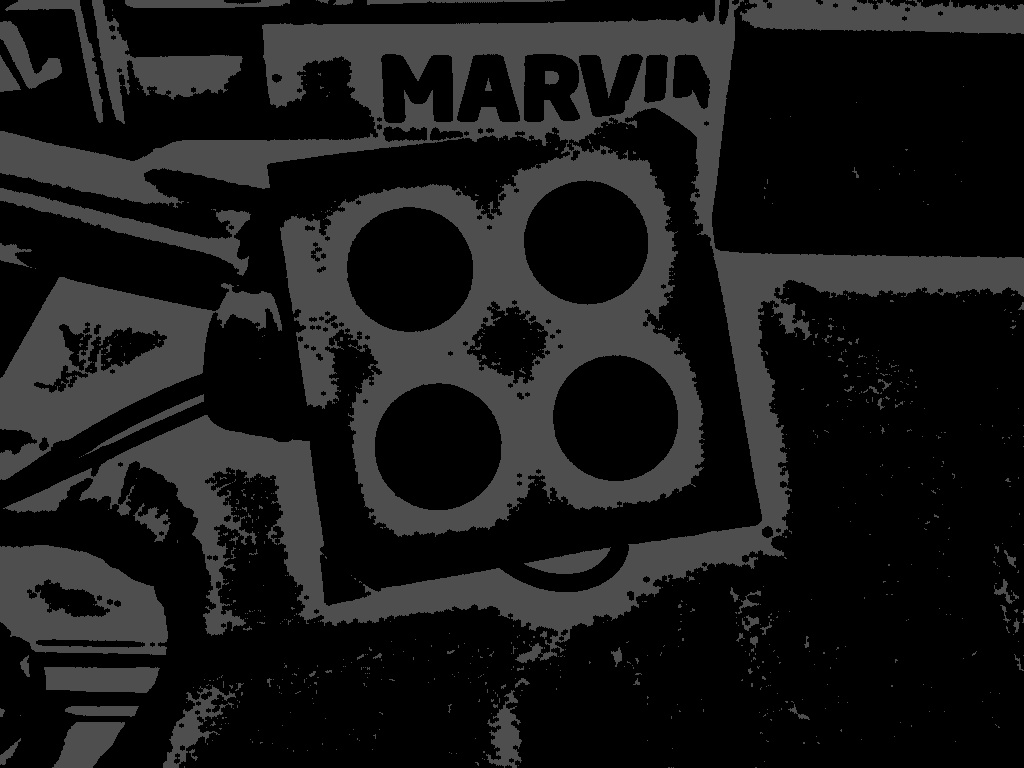
\includegraphics[width=0.8\textwidth]{circle_image_4}
    \caption{Eroded image}
\label{fig:circle_process_examples_4}
\end{subfigure}
\begin{subfigure}[b]{0.3\linewidth}
\centering
    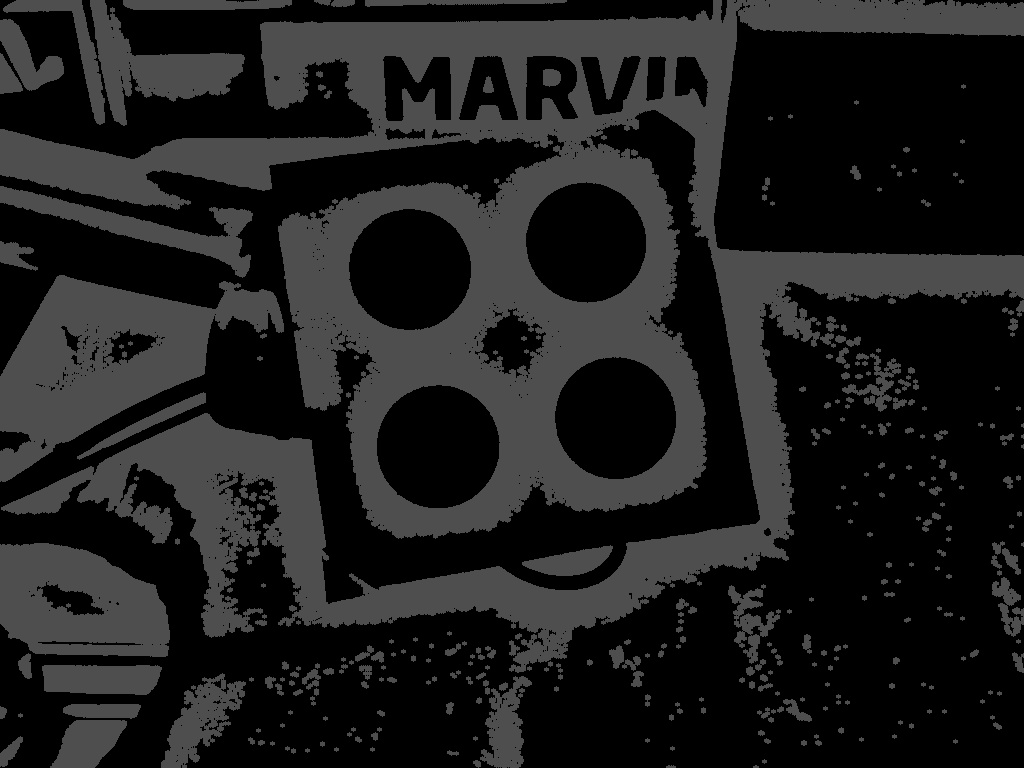
\includegraphics[width=0.8\textwidth]{circle_image_5}
    \caption{Dilated image}
\label{fig:circle_process_examples_5}
\end{subfigure}
\begin{subfigure}[b]{0.3\linewidth}
\centering
    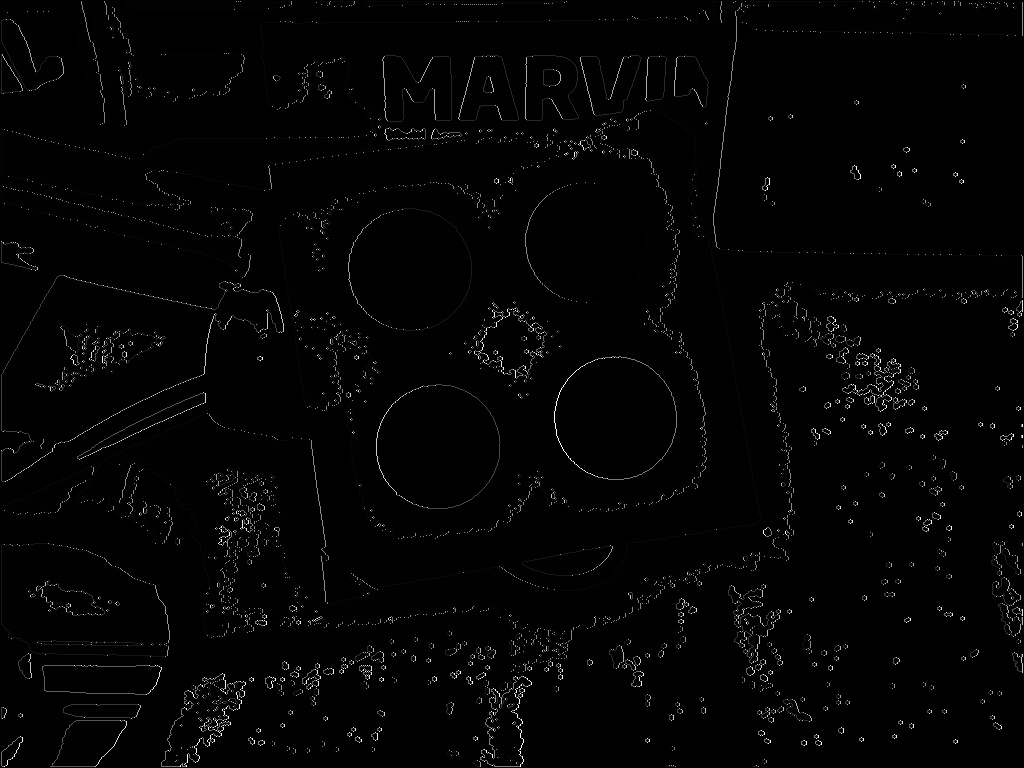
\includegraphics[width=0.8\textwidth]{circle_image_6}
    \caption{Thresholded image}
\label{fig:circle_process_examples_6}
\end{subfigure}\\
\begin{subfigure}[b]{0.9\linewidth}
\centering
    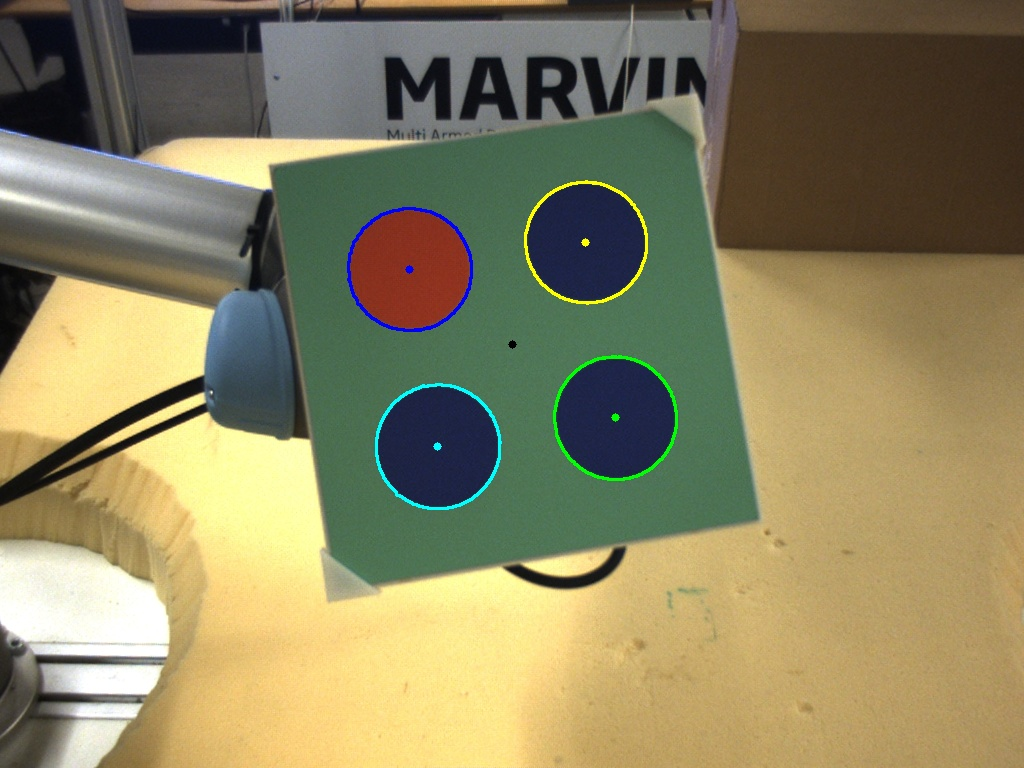
\includegraphics[width=0.2\textwidth]{circle_image_7}
    \caption{Found circles and center of marker (dark spot in the middle)}
\label{fig:circle_process_examples_7}
\end{subfigure}
\caption{Image preparation process}
\label{fig:circle_process_examples}
\end{figure}

After thresholding, the image is first \verb|erode|d then \verb|dilate|d (opened) in order to remove noise and to separate the circles from the border of the plate.
Then, the image is thresholded, as the adaptive threshold actually offsets the expected white color into a more gray color.

After the preparation, \verb|findContours| is called.
The contours are first filtered after area.
Then a ratio, calculated after the formula in Equation~\vref{eq:circle_ratio} as explained by Henrik Skov Midtiby as a good metric for finding circles, is calculated.
\begin{align}\label{eq:circle_ratio}
    \mathit{ratio} = \frac{4\times\pi\times\mathit{area}}{\mathit{perimeter}^2}
\end{align}
This ratio is used to sort the contours in ascending order; lower ratios before higher ratios.
A perfect circle (which is not possible in a picture due to the quadrilateral nature of pixels) would have a ratio of 1.
This is easily shown by inserting the formulae for perimeter and area of a circle in Equation~\ref{eq:circle_ratio}:

\begin{align}
    \mathit{ratio}_\mathit{circle}  &= \frac{4\times\pi\times(\pi\times r^2)}{(2\times\pi\times r)^2}\nonumber \\
                                    &= \frac{4\times\pi^2\times r^2}{4\times\pi^2\times r^2} = 1
\end{align}

Since a higher ratio means more circle-like, the four contours most like a circle is in the four last positions.
It is assumed that the circles are in these four positions, which they indeed are in all test images in both the easy and hard sequence.

Using a contour's moment, it is easy to calculate the center of mass for the contour.
This, since it is a circle, is the center of the circle.
An average of the four centers is the midpoint between the four circles and thus the middle of the marker.

The developed identification routine singles out each of the four circles and uniquely identifies them based on their position in the original marker (see Figure~\vref{fig:original_circle_marker}); red, top right, bottom left, bottom right.
The identification is as such not used for e.g.\ extracting pose or ``orientation''.

Finding the red circle is a matter of comparing the color of the four found circles.
The circle which has a red value higher than the other three is the red circle.
In this implementation, only a single pixel (the one in the middle) is used; a better implementation would be taking an average over a larger sample.
The circle opposite of the red circle will be the circle to which red has the highest distance.

Those were the program linewise quick ones.

Finding the last two circles are based on four scenarios, as seen in Figure~\vref{fig:marker_rotation}.
First, the scenario must be deduced from the x and y coordinates of the red and opposite circles.
Then, the coordinate of one of the circles must be compared to the coordinate of one or both of the identified circles.
Lastly, the two circles are identified.

\begin{figure}[ht]
\centering
\begin{subfigure}[b]{0.45\linewidth}
\centering
    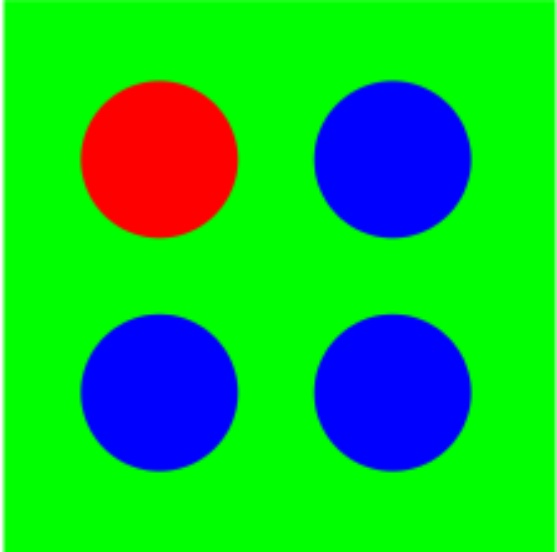
\includegraphics[width=0.7\textwidth]{circle_image_8}
    \caption{``Correct'' orientation}
\label{fig:marker_rotation_1}
\end{subfigure}
\begin{subfigure}[b]{0.45\linewidth}
\centering
    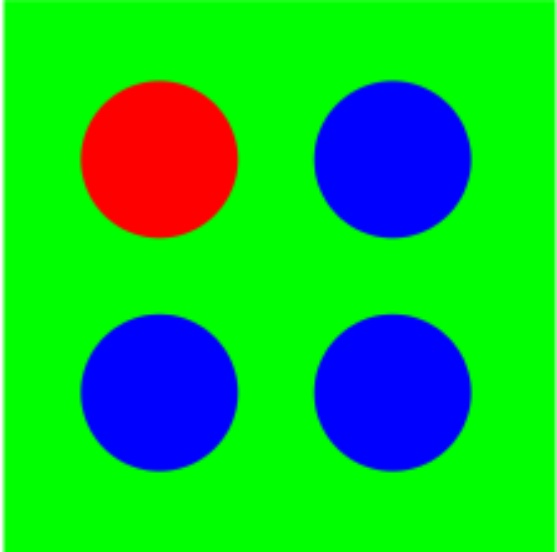
\includegraphics[angle=270, origin=c, width=0.7\textwidth]{circle_image_8}
    \caption{\SI{90}{\degree} rotation}
\label{fig:marker_rotation_2}
\end{subfigure}\\
\begin{subfigure}[b]{0.45\linewidth}
\centering
    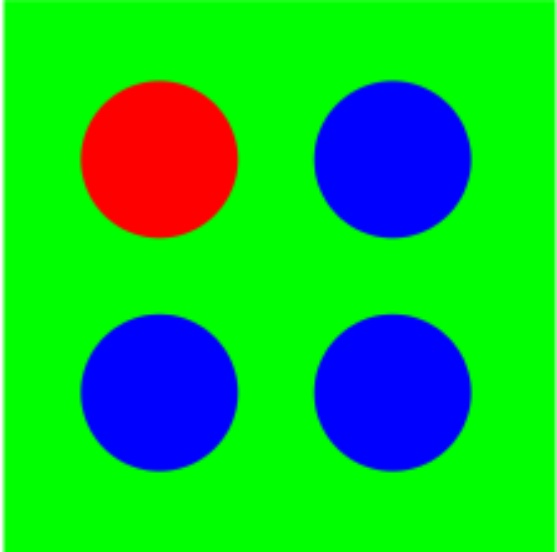
\includegraphics[angle=180, origin=c, width=0.7\textwidth]{circle_image_8}
    \caption{\SI{180}{\degree} rotation}
\label{fig:marker_rotation_3}
\end{subfigure}
\begin{subfigure}[b]{0.45\linewidth}
\centering
    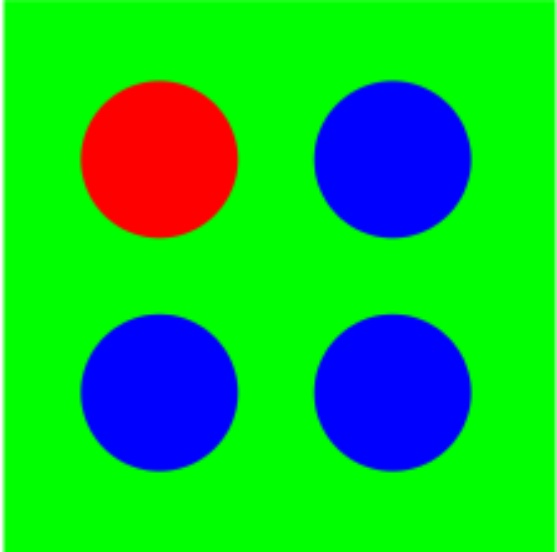
\includegraphics[angle=90, origin=c, width=0.7\textwidth]{circle_image_8}
    \caption{\SI{270}{\degree} rotation}
\label{fig:marker_rotation_4}
\end{subfigure}
\caption{Circle marker rotation cases}
\label{fig:marker_rotation}
\end{figure}

The whole process of loading an image storage, preparing image, searching for circles, identifying them,
finding midpoint of marker and returning that point can be done at \SI{>30}{\fps}.
The test machine is an Asus X53Sv laptop with an Intel Core i7--2630QM CPU @ 2.00GHz processor, \SI{8}{\giga\byte} RAM and a Samsung 850 EVO SSD.\@
Testing was performed immediately after a reboot.
The program correctly identifies the circles in every image.
